\chapter{Environment, Safety, and Health}
\label{vl:tc-ESH}


A strong \dword{esh} program is essential to successfully complete
\dword{lbnf} and \dword{dune} at \dword{surf} and hosted by
\fnal.  \dword{lbnf-dune} is internationally designed,
coordinated and funded through collaborating laboratories and
universities.  \dword{lbnf} comprises the
world's highest intensity neutrino beam at \fnal and the
infrastructure necessary to support the experimental detectors at
\dword{surf}. The \dword{dune} project is committed to ensuring a
safe work environment for \dword{dune} workers at all
institutions and to protecting the public from hazards associated with
constructing and operating \dword{dune}.  Accidents and
injuries are preventable, and we must work together to
establish a workplace free of injuries.  Finally, all work must be
performed so the quality of the environment is preserved
and property damage prevented.

\fnal and \dword{lbnf-dune} are committed to protecting the health and
safety of staff, the community and the environment, as stated in the
\dword{lbnf-dune} integrated \dword{esh} plan.  The
\dword{esh} program complies with applicable standards and local,
state and federal legal requirements through the \fnal work smart set
of standards and the contract between Fermi Research Alliance and the
\dword{doe} Office of Science (FRA-DOE). \fnal, as the host
laboratory, established the South Dakota Services Division to provide
facility support.  The South Dakota Services Division is responsible
for \dword{lbnf-dune} operations at \dword{surf}.

The \dword{lbnf-dune} \dword{esh} program strives to prevent
injuries or illness and seeks to continually improve safety and health
management.  To the maximum practical extent, all hazards must be
eliminated or minimized through substitution, engineering or
administrative controls.  Where engineering or administrative controls
are not feasible, \dword{ppe} must be used.

The \dword{lbnf-dune} \dword{esh} management system is
designed to work hand in hand with the \dword{surf} emergency
management systems to protect the public, workers and environment;
ensure compliance with the FRA-DOE contract and \fnal Work Smart
standards; and improve \fnal's and \dword{dune}'s ability to meet or
exceed customer expectations. Doing so helps in executing the
scientific mission.  \fnal uses a set of criteria to plan, direct,
control, coordinate, assure and improve how \dword{esh} policies,
objectives, processes and procedures are established, implemented,
monitored and achieved.

The \dword{lbnf} facilities at \dword{surf} are, moreover, subject to
the requirements of the \dword{doe} Workers Safety and Health Program,
Title 10, Code Federal Regulations, Part 851 (10 CFR 851). These
requirements are promulgated through the \fnal Director's Policy
Manual\footnote{\fnal Director's Policy Manual is:
  http://www.fnal.gov/directorate/Policy\_Manual.html}, and the \fnal
\dword{esh} Manual\footnote{\fnal ES\&H Manual is:
  http://esh.fnal.gov/xms/ESHQ-Manuals/feshm} (\dword{feshm}), which
align with the \dword{surf} \dword{esh} Manual.


\section{LBNF-DUNE ES\&H Management and Oversight}

The \dword{tcoord} and \dword{ipd} have responsibility for
implementation of the \dword{dune} \dword{esh} program.  The
\dword{lbnf-dune} \dword{esh} manager reports directly to the
\dword{tcoord} and \dword{ipd} and is responsible for providing
\dword{esh} support and oversight for development and implementation
\dword{lbnf-dune} \dword{esh} program. The \dword{dune} \dword{esh}
Coordinator report to the \dword{lbnf-dune} \dword{esh}
manager and have primary responsibility for \dword{esh} support and
oversight of the \dword{dune} \dword{esh} program for all activities
at collaborating institutions and at \dword{lbnf-dune}
facilities located at \dword{surf}.

Additional \dword{esh} Subject Matter Experts (SME) are available to provide
supplemental support to the project through the \fnal \dword{esh}
Section. The \fnal \dword{esh} Section, DOE-Fermilab Site Office, CERN and
\dword{surf} will provide supplemental \dword{esh} oversight to validate
implementation of the \dword{lbnf-dune} \dword{esh}  program.

The \dword{lbnf-dune} \dword{esh} Plan defines the \dword{esh}
requirements applicable to installation activities at the \dword{surf}
site. Regular \dword{esh} walkthroughs will be conducted by
\dword{lbnf-dune} \dword{esh} management personnel. All
findings will be documented utilizing the \fnal Predictive Solutions
database system.
Figure~\ref{fig:dune_esh} shows the \dword{lbnf-dune} \dword{esh} organization.
\begin{dunefigure}[LBNF-DUNE ES\&H]{fig:dune_esh}
  {The high level \dword{lbnf-dune} \dword{esh} organization.}
  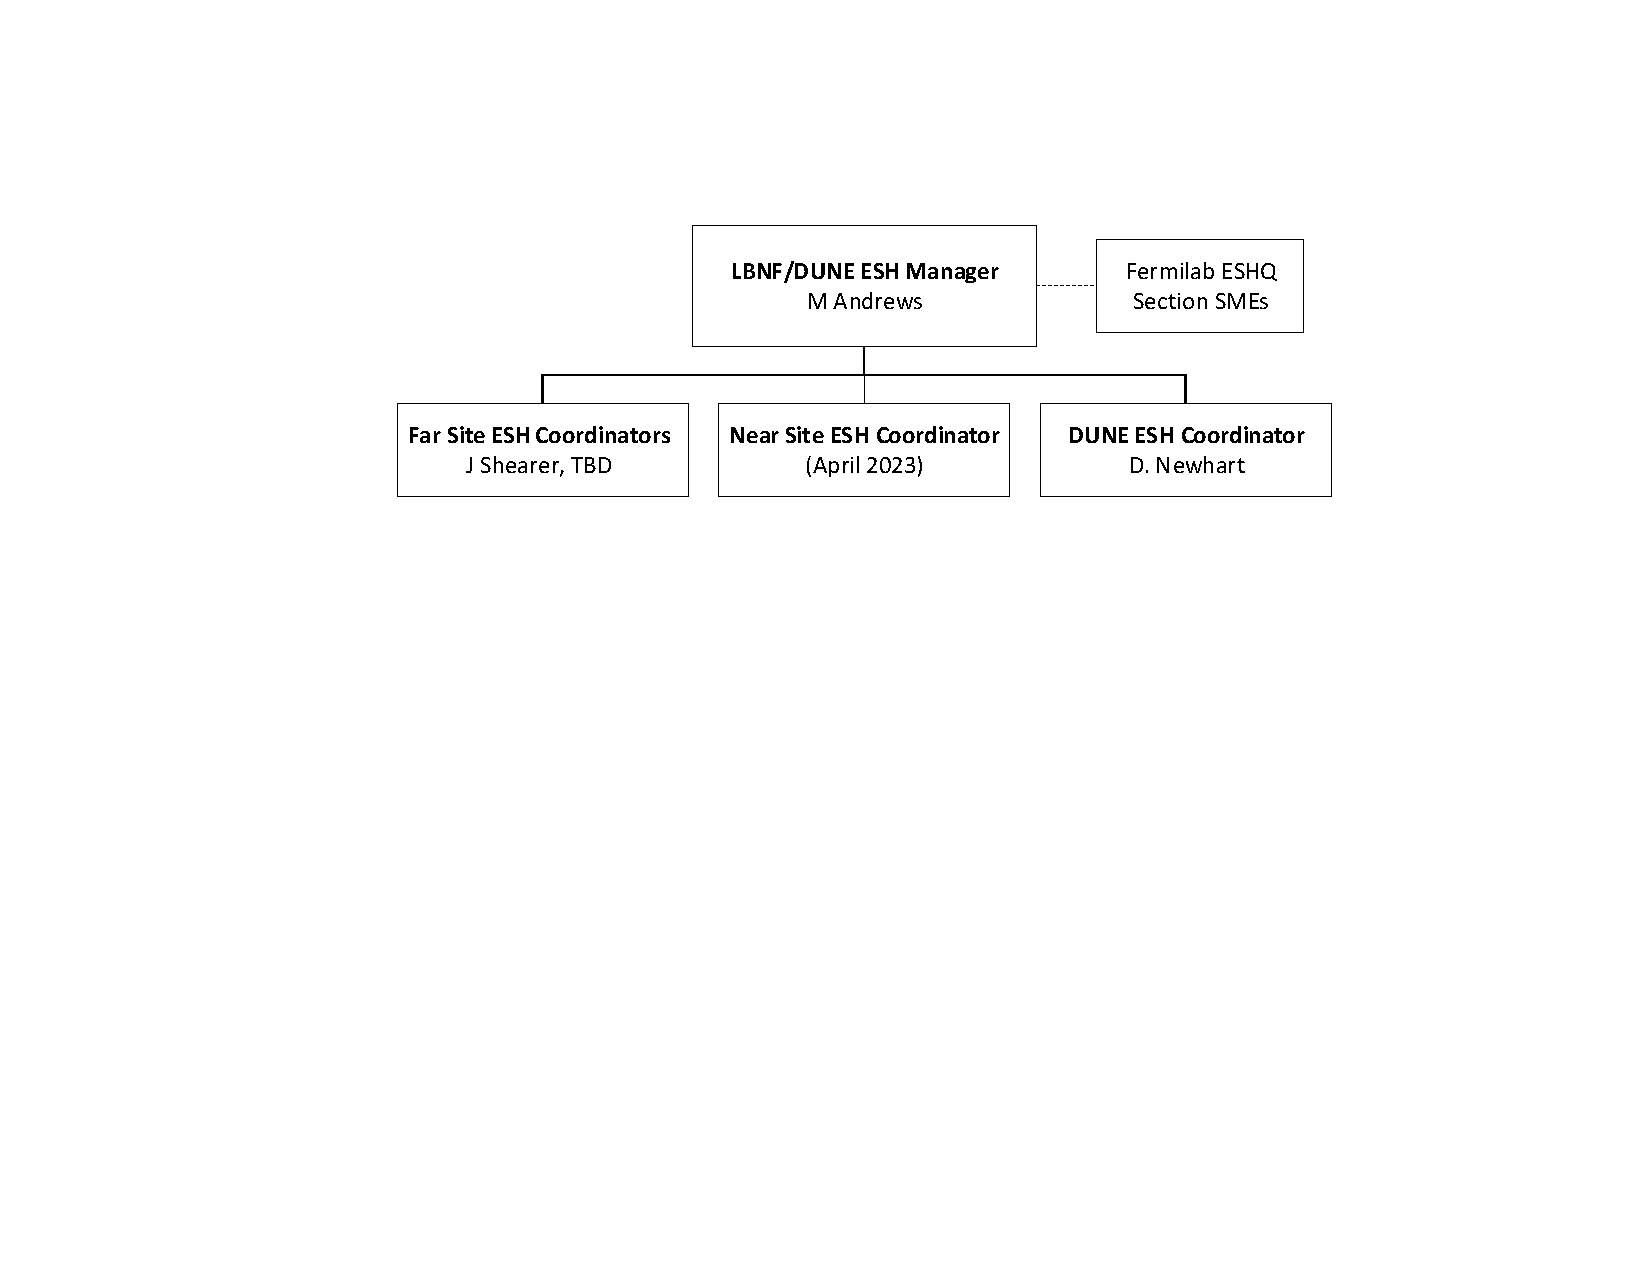
\includegraphics[width=0.85\textwidth]{ESH_ManagementandOversight_v2}
\end{dunefigure}

\section{National Environmental Protection Act Compliance}

In compliance with the National Environmental Protection Act and in
accordance with \dword{doe} Policy 451.1, the
\dword{lbnf-dune} project performed an evaluation of potential
environmental impacts during construction and operation of the
project.  An environmental assessment has been prepared on the
potential environmental impacts and the safety and health hazards
identified during the design, construction, and operating phases of
\dword{lbnf-dune}.  The environmental assessment presented an
analysis of the potential environmental consequences of the facility
and compared them to the consequences of a No Action Alternative. The
assessment included detailed analysis of all potential environmental,
safety, and health hazards associated with construction and operation
of the facility.  The environmental assessment has been completed and
a finding of no significant impact (FONSI) issued in September 2015.

\section{Codes/Standards Equivalencies}
\label{sec:esh_codes}

\dword{dune} will rely on significant contributions from international
partners. In many cases, an international partner will contribute
equipment for installation at \dword{fnal} built following one of the
international standards or directives. \dword{fnal} has established a
process, detailed in \dword{feshm} Chapter 2110, to establish code
equivalency between USA and international engineering design codes
and standards. This process allows the laboratory to accept in kind
contributions from international partners or purchase equipment
designed using international standards while ensuring an equivalent or
higher level of safety.

At the time of this writing, \fnal has completed the following code
equivalencies:
\begin{itemize}
 \item Pressure vessels designed using EN13445,
 \item Structures designed using EN 1990, EN 1991, EN1993, EN 1999 (a
   subset of the Eurocodes), and EN 14620;
 \item CE-marked pressure piping systems designed using PED 97/23 EN 13480;
 \item CE-marked relief valves designed using PED 2014/68/EU EN ISO 4126;
 \item CE-marked electrical equipment for measurement, control and
   laboratory use designed using IEC 61010-1 and IEC 61010-2-030.
\end{itemize}

As necessary, the laboratory code equivalency process will be followed
to establish equivalency to other international codes and
standards. The current list of completed code equivalencies can be
found in the \dword{esh}\&Q Section Document Database doc-3303
(https://esh-docdbcert.fnal.gov/cgi-bin/cert/ShowDocument?docid=3303).


\section{ES\&H Requirements at Collaborating Laboratories and Institutions}

All work performed at collaborating institutions will be completed
following that collaborating institutions \dword{esh} policies and
programs. Equipment and operating procedures provided by the
collaborating institution will conform to the \dword{dune} project
\dword{esh} and integrated safety management policies and
procedures. The \dword{esh} organization at collaborating institutions
must provide \dword{esh} oversight for all work activities carried
out at their institution facilities. \dword{lbnf-dune}
personnel will also follow the \dword{esh} manual and procedures at
the collaborating institutions.

\section{LBNF-DUNE ES\&H Program Requirements at SURF}

\subsection{Site and Facility Access}

All \dword{dune} workers requiring access to the \dword{surf} site must
register through the \fnal Users Office to receive the necessary user
training and a \fnal identification number. All workers must apply for
a \dword{surf} identification badge to access the \dword{surf} site as part of
the \dword{surf} Site Access Control Program.

\dword{surf} underground access will require that working groups
obtain a trip action plan (TAP) for each daily access to the
underground areas.  All personnel within each working group must be
individually listed on the trip action plan, per the \dword{surf} Site
Access Control Program. All personnel are required to ``brass in and
out'' via the brass board located at the entrance to the Ross Shaft
cage prior to accessing the underground facilities.

\subsection{ES\&H Training}

All \dword{dune} collaborators, as part of registration through the \fnal Users office,
will complete the user \dword{esh} training modules and the supervisor
will complete a training needs assessment to develop a training plan
to define additional \dword{dune} \dword{esh} training requirements.

\begin{comment}
All personal performing work on-site at \dword{surf} are required to
attend \dword{surf} \dword{esh} Site Orientation prior to performing
any work on-site.  The \dword{surf} Surface and Underground training
modules classes, including associated Cultural Heritage training, are
required to work on the site and arrangements will be made for all
workers to complete this training prior to beginning work. In
addition, unescorted access training will be provided to personnel for
each underground working level (4850L and 4910L) they will be required
to perform work.  The \dword{lbnf-dune} \dword{esh} management
team will present a project-specific introductory \dword{esh}
presentation.
\end{comment}
All personal performing work on-site at \dword{surf} are required to
attend \dword{surf} \dword{esh} Site Orientation prior to their work at the site.  This includes \dword{surf} Surface and Underground training classes, as well as associated Cultural Heritage training. Arrangements will be made for all workers to complete this training. In
addition, unescorted access training will be provided to personnel for
each underground working level (4850L and 4910L) at which they will perform work.  The \dword{lbnf}/\dword{dune} \dword{esh} management
team will present a project-specific introductory \dword{esh}
presentation.

\subsection{Personnel Protective Equipment}

Personal protective equipment (PPE) is not a substitute for
engineering and administrative controls. These controls shall be
implemented, to the extent feasible, to mitigate the hazard so that
the need for PPE is reduced or eliminated.

Personnel shall wear the following PPE when on site the \dword{surf} site.
\begin{itemize}
\item At a minimum, all workers personnel shall wear
  steel-toed boots, long pants and shirts with 4~inch sleeves when
  performing non-office work at \dword{surf}. 
  \item All personnel entering the work site at the Ross (or Yates) Dry
    shall wear hard hats (brim facing forward), gloves,
    safety glasses with rigid side-shields and reflective high
    visibility (e.g., orange) shirt/coat/vest (minimum ANSI Class 2).
    Exceptions to these minimum requirements shall be approved by the
    \dword{lbnf-dune} \dword{esh} manager and noted in the
    activity-specific \dword{ha} maintained by the \dword{lbnf-dune} \dword{esh} coordinator.
  \item When working underground, all personnel will carry an Ocenco M20.2 self rescuer
    and a hard hat cap lamp. In addition, Ocenco 7.5 emergency breathing apparatus devices
    will be stored underground for additional emergency support.
  \item Hard hats shall meet the ANSI Z89.1 standard as defined by 29
    CFR 1926.100 and bear the {\em Z89-.1} designation.
   \item Eye protection must meet the requirement of 29 CFR
      1926.102. Safety glasses must be ANSI approved and be marked
      with the ANSI marking {\em Z87.1} designation.
    \item Hearing protection appropriate to the work environment, as
      defined in the activity-based \dword{ha}.
    \item Any specialized PPE required for specific work tasks as
      defined in the activity-based \dword{ha}. 
\end{itemize}

\subsection{Work Planning and Controls}

The goal of the work planning and hazard analysis process is to
initiate thought about the hazards associated with work and how it can
be performed safely. Careful planning of a job assures that it is
performed efficiently and safely. Work planning ensures the scope of
the job is understood, appropriate materials are available, all
hazards have been identified, mitigation efforts established, and all
affected employees understand what is expected of them. Hazard
analysis is a critical part of work planning. All work activities
shall be subject to work planning and hazard analysis. Depending on
the complexity of the task and the hazards involved, the HA process
may be a mental exercise and verbal discussion, or it may be more
formal with a written hazard analysis and pre-job briefing. The Work
Planning and Hazard Analysis program is documented in Chapters 2060 in
the FESHM. All work planning documentation will be reviewed and
approved by \dword{dune} \dword{esh} Coordinator and the \dword{dune}
\dword{esh} Review Committee prior to the start of work activities.

A Work Planning Meeting shall be held each day/shift prior to the
start of daily work activities. The meeting(s) should be led by the
shift supervisor, supported by the \dword{dune} \dword{esh} Coordinator and
attended by all personnel working on-site that day. The duration of
the meetings is based on the activities occurring that day and
typically last approximately fifteen minutes. The daily planning
meetings should inform the workers of potential safety hazards and
hazard mitigations relating to the various work activities, ensure
that employees have the necessary \dword{esh} training and PPE, answer any
questions relating to the work activities and authorize the work
activities for that day.

A Safety Data Sheet (SDS) must be supplied for all chemicals and
hazardous materials that are used on site. All chemicals and hazardous
materials brought to the \dword{surf} site must be reviewed/approved by the
\dword{dune} \dword{esh} Coordinator and the \dword{surf} \dword{esh}
Department before arriving at site.  SDS documentation should be
submitted to the \dword{dune} \dword{esh} Coordinator prior to the
material arriving on site.

\subsection{Emergency Management}

Any injuries, accident or spill will be reported immediately to the
\dword{lbnf-dune} \dword{esh} manager. All personnel that
experience any injury will be sent or transported to the local clinic
or hospital as appropriate.  The supervisor shall complete an initial
Incident Investigation Report and submit the report to the
\dword{lbnf-dune} \dword{esh} manager within 24 hours.

For all emergencies at the \dword{surf} site, personnel shall contact
Emergency Response personnel by utilizing any building phone, dialing
the hoist operator or by calling 911 from any outside line (cell
phone).  \dword{surf} has a defined emergency response program on which all
personnel will be trained and the emergency notification process is
posted at all telephones.

SDSTA will maintain an Emergency Response incident command system and
an Emergency Response Team (ERT) on all shifts that should be able to
access the underground sites with normal surface fire department
response times. The Emergency Response Team has a defined training
schedule and emergency drills are conducted on both the surface and
underground sites, for which all personnel on site are required to
participate.

\dword{surf} implements a guide program for both the surface and
underground areas. The guide program has an established training
program. Guides are required to escort visitors/untrained personnel on
the \dword{surf} site. The underground guide program requires at a
minimum one guide on each working level underground to provide
supplemental emergency support to unescorted access trained
personnel. Guides are trained as first responders to help in a medical
emergency until the ERT arrives.

\subsection{Fire Protection, ODH and Life Safety}

The workforce shall police their work areas frequently and maintain
good housekeeping. Common garbage and other waste shall be disposed of
at frequent and regular intervals by the teams generating the
waste. Containers shall be provided for the collection and separation
of waste, trash, oily or used rags and other refuse.  Containers used
for garbage and other oily, flammable, or hazardous wastes, (such as
caustics, acids, harmful dusts or similar materials) shall be equipped
with covers.  Chemical agents or substances, which might react to
create a hazardous condition, shall be stored and disposed of
separately as assessed by the \dword{lbnf-dune} \dword{esh}
coordinator.

Chemicals and hazardous materials must be in proper storage cabinets
with SDS documentation readily available as collected by the
\dword{lbnf-dune} \dword{esh} coordinator. The
\dword{lbnf-dune} \dword{esh} coordinator will evaluate
appropriate storage cabinets for the \dword{ipd}.

Fermilab hot work permits shall be completed and approved for all open
flame, welding, cutting or grinding work activities.  The \dword{dune}
\dword{esh} Coordinator will coordinate the issuance of the permit.
The Subcontractor completing the work will be responsible for
providing all the required materials, personnel and protective
equipment to conduct all hot work. All hot work permits shall be
provided to the \dword{surf} \dword{esh} Department.

Cables installed for \dword{dune} are being chosen to be
consistent with current \fnal standards for cable insulation and
comply with recognized standards concerning cable fire resistance
reducing the probability of a fire starting and health effects of
combustion products of cable insulation materials.

Fire and life safety requirements for \dword{lbnf-dune} areas
were analyzed in the \dword{lbnf-dune} Far Site Fire and Life
Safety Assessment. All caverns will be equipped with fire detection
and suppression systems with both visual and audible notification. The
\dword{surf} will monitor all fire alarms and system supervisory signals in
the \dword{surf} Incident Command Center.  The \dword{surf} Emergency Response Team
will respond, with additional support from the Lead-Deadwood Fire
Department.

Oxygen Deficiency Hazards (ODH) requirements were assessed through the
\dword{lbnf-dune} ODH Analysis. The caverns will be equipped
with an ODH monitoring and alarm system with independent visual and
audible notification systems. \dword{surf} will monitor all ODH alarms and
system supervisory signals in the \dword{surf} Incident Command Center.

Emergency conditions from smoke or from ODH incidents underground are
primarily mitigated by the large ventillation rate in the \dword{surf}
underground area.

The facility emergency management plan will be developed for
installation and operation activities based on the egress strategy
defined in the ARUP Fire and Safety Report and the \dword{surf} Emergency
Management Plan.

\subsection{Material handling and Equipment Operation}

All overhead cranes, gantry cranes, fork lifts, motorized equipment,
e.g., trains and carts, will be operated only by trained
operators. Other equipment, e.g., scissor lifts, pallet jacks, hand
tools and shop equipment, will be operated only by personnel trained
for the particular piece of equipment. Such equipment will be powered
electrically or by diesel fuel, no other fuels are allowed. Diesel is
allowed due the large ventillation rate in the underground area.

Hoisting and rigging operations shall be evaluated and planned.  A
member of the trained rigging team shall identify the hazards and
determine the controls necessary to maintain an acceptable level of
risk.  A Hoisting and Rigging Lift Plan is required for complex and
critical lifts. This plan shall be documented using the \fnal Hoisting
and Rigging Lift Plan or similar plan accepted by \fnal. The Hazard
analysis documentation should also include the requirement for
development of critical lift plans for specific phases of demolition
or installation activities.

\subsection{Stop Work Authority}

If unanticipated/unsafe conditions are identified or non-compliant
practices are observed during construction activities, workers should
recognize that the work activity in which they are engaged should be
stopped and notify their supervisor and \dword{esh} officer of
this action. All workers on the \dword{dune} project have the
authority to stop work in any situation that presents an imminent
threat to safety, health and the environment. Work may not resume
until the circumstances are investigated and deficiencies corrected,
including the concurrence of the \dword{dune} \dword{ipd}
and \dword{lbnf-dune} \dword{esh} manager.

\subsection{Operationsal Readiness}

The \dword{dune} review process consists of design, production,
installation and operation reviews as described in
Chapter~\ref{vl:tc-review}. These reviews will include lifting fixture
load testing and work planning and controls documentation. The
\dword{jpo} Review Office is involved at all stages of the review
process. All major stakeholders (including \fnal, \dword{surf} and
\dword{dune} collaborating institutions) will be involved as
appropriate. The Review Office will complete both system and process
readiness reviews to authorize installation activities at
\dword{surf}.  Prior to operation of detector componentsvoperational
readiness reviews will be completed.

\subsection{Lessons Learned}

The \dword{lbnf} Project is currently working with SDSTA and the 
engineering consultant ARUP to implement \dword{esh} procedures and
protocols for site access, training, emergency management, fire
protection and life safety. The \fnal \dword{esh} Section, DOE and
\dword{lbnf} \dword{esh} have completed a series of assessments of
critical SDSTA \dword{esh} programs including underground access,
emergency management, electrical safety, rigging and fire
protection. The findings and lessons learned identified in these
\dword{esh} program assessments are tracked within the \fnal issues management
database --- iTrack.

The \dword{dune} team is comprised of experienced personnel from many
previous projects and \dword{protodune}.  \fnal completed a review to
identify critical lessons learned from the previous underground
neutrino project NuMI/MINOS Project in May 2009. The findings from this
exercise were documented in a report entitled Executive Summary of
Major NuMI Lessons Learned.  \dword{dune} lessons learned from
\dword{protodune} are being utilized to further develop and enhance
the \dword{dune} engineering review and work planning and controls
processes.

Lessons learned are disseminated in areas of applicability and
flowed-down for appropriate implementation. Any action items
associated with lessons learned are tracked in iTrack. Lessons learned
are reviewed and evaluated by both \fnal and \dword{lbnf-dune} management.

The \dword{lbnf} Project is presently implementing \dword{esh}
programs required for site access, training, work planning and
emergency management for construction activities on the \dword{surf}
site. During the implementation of these program lessons learned will
be identified and addressed to improve the implementation of the \dword{lbnf-dune}
\dword{esh} programs.  The \dword{esh} programs will be fully
established and implemented when \dword{dune} activities start at
\dword{surf}.
